% MAIN DOCUMENT

% change meta text values in ./meta/parameters.tex
% save chapters and corresponding data in ./chapters/XX/
% save images in ./images/
% remove ./example/ from the project root and clear references in this file
% add imports to ./meta/packages.tex, only if necessary

% version from 2024-03



\documentclass[a4paper, oneside, 11pt]{book}
\usepackage[utf8]{inputenc}

\newif\ifdraft
\drafttrue												% flag: marks document as draft and shows to-do-notes, comment or set to "draftfalse"

% PACKAGE IMPORTS



% compilation packages
%\usepackage{morewrites}                                  			% set more write registers, default: 16
																	% -> use when: "No room for a new \write."
%\usepackage{silence}												% suppress warnings
																	% -> use when: /



% general packages
\usepackage[top=2.5cm, bottom=2cm, left=3cm, right=2cm]{geometry}   % set page margins
\usepackage[ngerman]{babel}                                         % set language
\usepackage[T1]{fontenc}                                            % set font encoding
\usepackage[nottoc,notlot,notlof]{tocbibind}                        % remove toc, lot and lof from table of contents
\usepackage[bottom]{footmisc}                                       % set footnotes to bottom of page
\usepackage{setspace}                                               % set line spacing
\usepackage{parskip}                                                % set paragraph spacing
\usepackage{graphicx}                                               % include graphics
\usepackage{etoolbox}                                               % patch commands
\usepackage{fancyhdr}                                               % set header and footer
\usepackage{titlesec}                                               % set title format
\usepackage[titles]{tocloft}                                        % set table of contents format
\usepackage{csquotes}                                               % set quotation marks
\usepackage[
	backend=biber,					% biber package for compilation
	citestyle=numeric,				% citation style matching: IEEE
	bibstyle=numeric,				% citation style matching: IEEE
	sorting=none,					% sorting: as in document: IEEE
	%title={Literaturverzeichnis}	% title of bibliography
]{biblatex}															% set bibliography format
\usepackage[pdftex, pdfborder={0 0 0}]{hyperref}                    % set hyperlinks
\usepackage{lmodern}                                                % set font
\usepackage{color}                                                  % set colors
\usepackage{xcolor}                                                 % set colors
\usepackage{xspace}                                                 % set spaces
\usepackage{caption}                                                % set caption format
\usepackage{tabulary}                                               % set tables
\usepackage[acronym, toc]{glossaries}						   		% set glossaries and acronyms



% TColorbox packages
% -> documentation: https://texdoc.org/serve/tcolorbox/0
\usepackage{shellesc}												% required for shell escape
\usepackage{tcolorbox}												% required for creating colored boxes
\usepackage{fontawesome}											% required for using icons
\usepackage{minted}													% required for code listing and syntax highlighting
																	% -> requires shell escape !
\tcbuselibrary{skins}												% required for creating custom skins
\tcbuselibrary{most}												% required for using most features
\tcbuselibrary{minted}												% required for using minted
\tcbuselibrary{breakable} 										 	% required for breaking boxes



% additional packages for development
\usepackage{comment}												% enable comments in source code
\ifdraft
	\usepackage{todonotes}                                          % enable notes
\else
	\usepackage[disable]{todonotes}                                 % disable
\fi
%\usepackage{showframe} 	                                        % show layout borders									% import packages
% PARAMETERS FOR METADATA



% general metadata concerning the scientific work
\newcommand{\documentCategory}{Projekt\xspace}
\newcommand{\course}{Modul\xspace}
\newcommand{\courseAbbreviation}{AKRNM\xspace}
\newcommand{\semester}{(W|S)S-JJJJ[/YYYY]\xspace}
\newcommand{\project}{Projekttitel oder -kurzbeschreibung\xspace}

% flag for single or group work
% note: there is no integrity check for the students, 
%       meaning that more than one student can be set to true although the work is set to single, or vice versa
\newboolean{singleAuthor} \setbool{singleAuthor}{true}

% flags for enabling the visibility of authors
\newboolean{studentA} \setboolean{studentA}{true}
\newboolean{studentB} \setboolean{studentB}{false}
\newboolean{studentC} \setboolean{studentC}{false}
\newboolean{studentD} \setboolean{studentD}{false}
\newboolean{studentE} \setboolean{studentE}{false}
\newboolean{studentF} \setboolean{studentF}{false}

% metadata concerning the authors
\newcommand{\studentAName}{Studierende oder Studierender\xspace}
\newcommand{\studentAMatNr}{00000000\xspace}
\newcommand{\studentBName}{Studierende oder Studierender\xspace}
\newcommand{\studentBMatNr}{00000000\xspace}
\newcommand{\studentCName}{Studierende oder Studierender\xspace}
\newcommand{\studentCMatNr}{00000000\xspace}
\newcommand{\studentDName}{Studierende oder Studierender\xspace}
\newcommand{\studentDMatNr}{00000000\xspace}
\newcommand{\studentEName}{Studierende oder Studierender\xspace}
\newcommand{\studentEMatNr}{00000000\xspace}
\newcommand{\studentFName}{Studierende oder Studierender\xspace}
\newcommand{\studentFMatNr}{00000000\xspace}

% flags for enabling the visibility of tutors
\newboolean{tutorA} \setboolean{tutorA}{true}
\newboolean{tutorB} \setboolean{tutorB}{true}

% metadata concerning the tutor
\newcommand{\tutorAName}{Dozentin oder Dozent\space}
\newcommand{\tutorBName}{Betreuerin oder Betreuer\space}

% metadata concerning the document
\newcommand{\documentDayOfWeek}{Wochentag\xspace}
\newcommand{\documentDay}{TT\xspace}
\newcommand{\documentMonth}{MM\xspace}
\newcommand{\documentMonthOfYear}{Monat\xspace}
\newcommand{\documentYear}{JJJJ\xspace}
\newcommand{\documentDate}{\documentDayOfWeek, \documentDay.\documentMonth.\documentYear\xspace}

% metadata concerning the university
\newcommand{\university}{Ostfalia Hochschule für angewandte Wissenschaften \\
                         Hochschule Braunschweig / Wolfenbüttel\xspace}
\newcommand{\faculty}{Informatik\xspace}
\newcommand{\degree}{Bachelor of Science (B.Sc.)\xspace}
\newcommand{\studies}{Informatik\xspace}

% metadata required if the document is a thesis
\newboolean{thesis} \setboolean{thesis}{false}

% metadata concerning the document manager (default: first student)
\newcommand{\firstAuthor}{\studentAName\xspace}								% set meta parameters
% COMMANDS FOR METATEXT



% title of the document (derived from document category)
\newcommand{\documentTitle}{\documentCategory\xspace}

% subtitle of the document (derived from project title)
\newcommand{\documentSubtitle}{\projectdescription\xspace}

% subject of the document (derived from course and semester)
\newcommand{\documentSubject}{\course (\courseAbbreviation), \\\semester\xspace}

% authors of the document (derived from student data, if set to visible)
\newcommand{\documentAuthor}{
    \ifbool{studentA}  {\studentAName, Mat.-Nr.: \studentAMatNr}{}
    \ifbool{studentB}{\\\studentBName, Mat.-Nr.: \studentBMatNr}{}
    \ifbool{studentC}{\\\studentCName, Mat.-Nr.: \studentCMatNr}{}
    \ifbool{studentD}{\\\studentDName, Mat.-Nr.: \studentDMatNr}{}
    \ifbool{studentE}{\\\studentEName, Mat.-Nr.: \studentEMatNr}{}
    \ifbool{studentF}{\\\studentFName, Mat.-Nr.: \studentFMatNr}{}
    \xspace
}

% lecturer of the document (derived from tutor)
\newcommand{\documentTutor}{\tutor\xspace}

% signature fields for single author
\newcommand*{\SignatureAndDate}[1]{
    
	\par\noindent\makebox[52mm]{\hrulefill} \hfill\makebox[65mm]{\hrulefill}
	\par\noindent\makebox[52mm][c]{Ort, Datum} \hfill\makebox[62mm][c]{#1}
    \xspace
}									% define custom commands and environments
% PAGE LAYOUT
% requires packages from "packages.tex"



\selectlanguage{ngerman}								% set language to german

\setlength{\parindent}{0em} 							% paragraph indentation to left-justified

\onehalfspacing											% set line spacing to 1.5

\makeatletter

% configure headers
\patchcmd{\@makechapterhead}{\vspace*{50\p@}}{}{}{} 	% removes space above \chapter head
\patchcmd{\@makeschapterhead}{\vspace*{50\p@}}{}{}{} 	% removes space above \chapter* head
\makeatother
\setlength{\headheight}{14.5pt}							% set header height
\pagestyle{fancy}										% set page style to fancy
\renewcommand{\chaptermark}[1]{							% set chapter mark
	\markboth{
		{\chaptername\ \thechapter\ #1}
	}{}
}
\renewcommand{\sectionmark}[1]{							% set section mark
	\markright{
		{\projectshortdescription}
	}
}

\fancypagestyle{titlepage}								% set title page style
{
	\setcounter{page}{-100000}
	\fancyhf{}
	\fancyfootoffset{0pt}
	\fancyheadoffset{0pt}
	\renewcommand{\headrulewidth}{0pt}
}

% set fonts of titles
\titleformat{\chapter}[display] {\sffamily \huge}{\chaptertitlename\ \thechapter}{-5pt}{\Huge}
\titlespacing*{\chapter}{0pt}{0pt}{10pt}
\titleformat{\section}[display] {\sffamily \tiny}{}{0pt}{\LARGE \thesection\ }
\titlespacing*{\section}{0pt}{0pt}{0pt}
\titleformat{\subsection}[display] {\sffamily \tiny}{}{-15pt}{\Large \thesubsection\ }
\titlespacing*{\subsection}{0pt}{0pt}{0pt}
\titleformat{\subsubsection}[display] {\sffamily \tiny}{}{-15pt}{\large \thesubsubsection\ }
\titlespacing*{\subsubsection}{0pt}{0pt}{0pt}

% set fonts of table of contents
\renewcommand{\cftchapfont}{\bf\sffamily}
\renewcommand{\cftsecfont}{\sffamily}
\renewcommand{\cftsubsecfont}{\sffamily}

% set fonts of footnotes
\renewcommand{\cfttabfont}{\sffamily}
\renewcommand{\cftfigfont}{\sffamily}

\setcounter{secnumdepth}{3}

% set metadata of document
\hypersetup{
	pdfauthor={\firstAuthor},
	pdftitle={\documentTitle\ | \documentSubtitle},
	pdfsubject={\documentSubject},
	pdfkeywords={Betreuer: \tutorAName}
}

% set code listings
\lstset{
	showspaces=false,
	showtabs=false,
	breaklines=true,
	showstringspaces=false,
	basicstyle=\ttfamily,
	frame=lt,
	rulecolor=\color{gray},
	framerule=3pt,
	xleftmargin=6pt,
}

% set code boxes
\newtcblisting{codebox}[3][]{%
	listing engine=minted,
	minted style=colorful,
	minted language=#2,
	minted options={tabsize=2,breaklines,autogobble,linenos,numbersep=3mm},
	colback=white,
	colframe=darkgray,
	listing only,
	left=5mm,
	title=\faCode\quad #3,
	enhanced,
	overlay={\begin{tcbclipinterior}\fill[lightgray] (frame.south west)
	rectangle ([xshift=5mm]frame.north west);\end{tcbclipinterior}},
	#1
}

% style captions
\newlength\myx
\setlength\myx{\textwidth}
\addtolength\myx{-2\fboxsep}
\DeclareCaptionFont{white}{\color{white} \sffamily}
\DeclareCaptionFormat{listing}{\colorbox{gray}{\parbox{\myx}{#1#2#3}}}
\captionsetup[lstlisting]{format=listing,labelfont=white,textfont=white}
\renewcommand{\lstlistingname}{Quelltext}									% set document header and page layout
% hyphenation								% define hyphenation rules

\setcounter{chapter}{-1}								% reset chapter counter to start with 0

\addbibresource{literature.bib}							% import bibliography

\begin{document}

	%-------------------------------------------------------------------------------
	% COVER, TOC, AFFIDAVIT
	%-------------------------------------------------------------------------------

	\listoftodos
	% COVER PAGE



\frontmatter
\begin{titlepage}
\thispagestyle{titlepage}

    %---------------------------------------------------------------------------

    \newgeometry{top=2cm, bottom=3.5cm, left=1.5cm, right=1.5cm}

    \hfill
    \includegraphics[scale=0.93]{logos/logo_ostfalia.jpg}
    \includegraphics[scale=1.20]{logos/sublogo_wf.jpg}

    \vspace{0.5em}
    \hspace{1cm}
    \begin{minipage}{\dimexpr\textwidth-1.5cm\relax}
        {\Large\textsf{Fakultät \faculty}}
    \end{minipage}

    \vfil

    %---------------------------------------------------------------------------

    \hspace{1cm}
    \begin{minipage}{\dimexpr\textwidth-1.5cm\relax}
        \hrulefill

        \vspace{2em}

        {\LARGE\textbf{\textsf{\documentSubject\documentYear}}}

        \vspace{2em}

        {\Huge\textbf{\textsf{\documentTitle}}}

        \vspace{2em}

        {\Large\textsf{\documentSubtitle}}

        \vspace{1em}

        \hrulefill
    \end{minipage}

    %---------------------------------------------------------------------------

    \vfil

    \begingroup
    \centering
    \ifbool{thesis}{
        \textsf{
            Zur Erlangung des akademischen Grades\\
            \textbf{\degree}\\
            im Studiengang \studies\\
            an der\\
            \university\\
        }
    }{}
    \endgroup

    %----------------------------------------------------------------------------

    \vfil

    \hspace{1cm}
    \begin{minipage}{\dimexpr\textwidth-1.5cm\relax}
        {\Large\textsf{
            \ifbool{thesis}{
                vorgelegt von \\\textbf{\documentAuthor}
            }{
                \textbf{Autor\ifbool{singleAuthor}{}{en}:} \\\documentAuthor
            }}}

        \vspace{0.5cm}

        {\Large\textsf{
            \textbf{Betreuende:}
            \ifbool{tutorA}{\\\tutorAName}{}
            \ifbool{tutorB}{\\\tutorBName}{}
        }}

        \vspace{0.5cm}

        {\Large\textsf{
            \textbf{Abgabedatum:} \\\documentDate
        }}
    \end{minipage}

    \vfil

    %---------------------------------------------------------------------------

    \enlargethispage{5\baselineskip}

    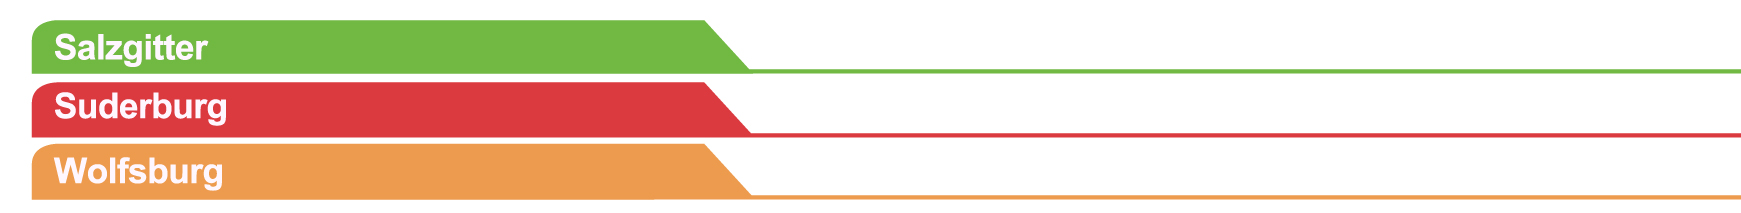
\includegraphics[scale=1.20]{logos/sublogo_sz-sud-wob.jpg}

    %---------------------------------------------------------------------------

\end{titlepage}

\restoregeometry
	
	\tableofcontents
	\listoffigures
	\listoftables
	
	\chapter*{Erklärung}

\ifbool{singleAuthor}{
    Hiermit versichere ich, die vorliegende Arbeit selbständig verfasst und keine anderen als die angegebenen Quellen und Hilfsmittel verwendet zu haben. Ich versichere weiterhin, alle wörtlich oder sinngemäß aus anderen Quellen übernommenen Aussagen als solche gekennzeichnet zu haben. Dies gilt explizit auch für die Verwendung von text- oder codegenerierenden Werkzeugen der Künstlichen Intelligenz.
    Die eingereichte Arbeit ist weder vollständig noch in wesentlichen Teilen Gegenstand eines anderen Prüfungsverfahrens gewesen.
    Ich habe zur Kenntnis genommen, dass die Arbeit einer elektronischen Plagiatsprüfung unterzogen werden kann.
}{
    Hiermit versichern wir, die vorliegende Arbeit selbständig verfasst und keine anderen als die angegebenen Quellen und Hilfsmittel verwendet zu haben. Wir versichern weiterhin, alle wörtlich oder sinngemäß aus anderen Quellen übernommenen Aussagen als solche gekennzeichnet zu haben. Dies gilt explizit auch für die Verwendung von text- oder codegenerierenden Werkzeugen der Künstlichen Intelligenz.
    Die eingereichte Arbeit ist weder vollständig noch in wesentlichen Teilen Gegenstand eines anderen Prüfungsverfahrens gewesen.
    Wir haben zur Kenntnis genommen, dass die Arbeit einer elektronischen Plagiatsprüfung unterzogen werden kann.
}

\vspace*{3em}

\ifbool{studentA}{\SignatureAndDate{- \studentAName\ -}}{} \\\\
\ifbool{studentB}{\SignatureAndDate{- \studentBName\ -}}{} \\\\
\ifbool{studentC}{\SignatureAndDate{- \studentCName\ -}}{} \\\\
\ifbool{studentD}{\SignatureAndDate{- \studentDName\ -}}{} \\\\
\ifbool{studentE}{\SignatureAndDate{- \studentEName\ -}}{} \\\\
\ifbool{studentF}{\SignatureAndDate{- \studentFName\ -}}{} \\
	
	%-------------------------------------------------------------------------------
	% CONTENT
	%-------------------------------------------------------------------------------

	\mainmatter
	
	\chapter{Einleitung und Motivation}
\label{ch:00-introduction-and-motivation}

Als Teil der Bewertung des Moduls \flqq \course (\courseAbbreviation)\frqq\xspace ist diese Ausarbeitung Gegenstand der Prüfungsaufgabe zum \semester. Sie enthält die Dokumentation der in \ifbool{singleAuthor}{Einzelarbeit}{Gruppenarbeit} erstellten Entwicklungsaufgabe und knüpft damit in großen Teilen an die in dem Modul erarbeiteten Inhalte an.

Zum Zweck der besseren Lesbarkeit wird in dieser Abhandlung größtenteils auf die geschlechtsspezifische Schreibweise verzichtet.
Das gewählte generische Maskulinum bezieht sich jedoch immer zugleich auf weibliche und männliche Personen, sofern dies für die Aussage erforderlich ist.\\

%replace text with content here
Beschreibung der Projektaufgabe\\

%replace text with content here
Benennung der Projektziele\\
	\chapter{Kapitel}
\label{ch:01-chapter}

% replace text with content here
Inhalt
	\chapter{Vorlage}

Einleitung



\section{Sektion}

Text



\subsection{Subsektion}

Text



\section{Fazit}

Text				% template for new chapters, remove from main
	\chapter{Kapitel}

\section{Beispiel 0}

\subsection{Unterpunkt}
\enquote{Das ist ein Beispielzitat.} \footnote{Fußnote}

Das ist ein Beispieltext. Das ist ein Beispieltext. Das ist ein Beispieltext. Das ist ein Beispieltext. Das ist ein Beispieltext. Das ist ein Beispieltext. Das ist ein Beispieltext. Das ist ein Beispieltext. Das ist ein Beispieltext. Das ist ein Beispieltext. Das ist ein Beispieltext. Das ist ein Beispieltext. Das ist ein Beispieltext. Das ist ein Beispieltext. Das ist ein Beispieltext.

\begin{figure}
	\centering
	\includegraphics{./images/logos/logo_ostfalia.jpg}
	\caption{Bild}
\end{figure}

\subsubsection{Unterunterpunkt}
Das ist ein Beispieltext. Das ist ein Beispieltext. Das ist ein Beispieltext. Das ist ein Beispieltext. Das ist ein Beispieltext. Das ist ein Beispieltext. Das ist ein Beispieltext. Das ist ein Beispieltext. Das ist ein Beispieltext. Das ist ein Beispieltext. Das ist ein Beispieltext. Das ist ein Beispieltext. Das ist ein Beispieltext. Das ist ein Beispieltext. Das ist ein Beispieltext.

Das ist ein Beispieltext. Das ist ein Beispieltext. Das ist ein Beispieltext. Das ist ein Beispieltext. Das ist ein Beispieltext. Das ist ein Beispieltext. Das ist ein Beispieltext. Das ist ein Beispieltext. Das ist ein Beispieltext. Das ist ein Beispieltext. Das ist ein Beispieltext. Das ist ein Beispieltext. Das ist ein Beispieltext. Das ist ein Beispieltext. Das ist ein Beispieltext.

\subsection{Fazit}
Das ist ein Fazit. Das ist ein Fazit. Das ist ein Fazit. Das ist ein Fazit. Das ist ein Fazit. Das ist ein Fazit. Das ist ein Fazit. Das ist ein Fazit. Das ist ein Fazit. Das ist ein Fazit. Das ist ein Fazit. Das ist ein Fazit. Das ist ein Fazit. Das ist ein Fazit. Das ist ein Fazit.

Das ist ein Fazit aus einer Referenz. Das ist ein Fazit aus einer Referenz. Das ist ein Fazit aus einer Referenz. Das ist ein Fazit aus einer Referenz. Das ist ein Fazit aus einer Referenz. Das ist ein Fazit aus einer Referenz. Das ist ein Fazit aus einer Referenz. Das ist ein Fazit aus einer Referenz. Das ist ein Fazit aus einer Referenz. Das ist ein Fazit aus einer Referenz. Das ist ein Fazit aus einer Referenz. Das ist ein Fazit aus einer Referenz. Das ist ein Fazit aus einer Referenz. Das ist ein Fazit aus einer Referenz. Das ist ein Fazit aus einer Referenz. \cite{000:Reference}

Das ist ein Fazit aus einer weiteren Referenz. \cite{001:Reference}

\begin{table}
	\centering
	\begin{tabular}{| l c r |}
		\hline
		1 & 2 & 3 \\
		4 & 5 & 6 \\
		7 & 8 & 9 \\
		\hline
	\end{tabular}
	\caption{Tabelle}
\end{table}

\section{Beispiel 1}

\subsection{Unterpunkt}
Hier ist Platz für Text. Hier ist Platz für Text. Hier ist Platz für Text. Hier ist Platz für Text. Hier ist Platz für Text. Hier ist Platz für Text. Hier ist Platz für Text. Hier ist Platz für Text. Hier ist Platz für Text. Hier ist Platz für Text. Hier ist Platz für Text. Hier ist Platz für Text. Hier ist Platz für Text. Hier ist Platz für Text. Hier ist Platz für Text. Hier ist Platz für Text. Hier ist Platz für Text. Hier ist Platz für Text. Hier ist Platz für Text. Hier ist Platz für Text. Hier ist Platz für Text. Hier ist Platz für Text. Hier ist Platz für Text. Hier ist Platz für Text. Hier ist Platz für Text. Hier ist Platz für Text. Hier ist Platz für Text. Hier ist Platz für Text. Hier ist Platz für Text. Hier ist Platz für Text. Hier ist Platz für Text. Hier ist Platz für Text. Hier ist Platz für Text. Hier ist Platz für Text. Hier ist Platz für Text. Hier ist Platz für Text. Hier ist Platz für Text. Hier ist Platz für Text. Hier ist Platz für Text. Hier ist Platz für Text. Hier ist Platz für Text. Hier ist Platz für Text. Hier ist Platz für Text. Hier ist Platz für Text. Hier ist Platz für Text. Hier ist Platz für Text. Hier ist Platz für Text. Hier ist Platz für Text. Hier ist Platz für Text. Hier ist Platz für Text. 

\subsection{Fazit}
Das ist ein Fazit. Das ist ein Fazit. Das ist ein Fazit. Das ist ein Fazit. Das ist ein Fazit. Das ist ein Fazit. Das ist ein Fazit. Das ist ein Fazit. Das ist ein Fazit. Das ist ein Fazit. Das ist ein Fazit. Das ist ein Fazit. Das ist ein Fazit. Das ist ein Fazit. Das ist ein Fazit.

\missingfigure{Hier fehlt ein Element.}

Hier ist weiterer Text, entnommen aus einer Referenz. \cite{000:Reference}

\lstinputlisting[caption={Code-Beispiel},float,language=Html]{chapters/example/example.html}

Hier ist weiterer Text ohne Referenz.

\lstinputlisting[caption={Some Code},float,language=Java]{chapters/example/Example.java}

Hier ist weiterer Text.

Hier ist weiterer Text.					% example chapter, remove from main
	\chapter{Schluss und Fazit}
\label{ending-and-conclusion}

%replace text with content here
Schluss und Fazit

	%---------------------------------------------------------------------------
	% BIBLIOGRAPHY
	%---------------------------------------------------------------------------

	\clearpage
	\renewcommand{\bibname}{Literaturverzeichnis}		% set bibliography title, default: Literatur
	\addcontentsline{toc}{chapter}{Literaturverzeichnis}
	\printbibliography
	
	\clearpage

	%---------------------------------------------------------------------------
	% APPENDIX
	%---------------------------------------------------------------------------

	\appendix
	\pagenumbering{Roman}
	\chapter{Anhang A}
\label{attachment-a}

% clear page only when including larger objects that otherwise would result in a page break in the middle of the object
\textit{siehe nächste Seite}\\\\
Der Anhang enthält auf den nächsten Seiten [...].
\clearpage

% for plain text
%Text

% for PDF-Files
%\includepdf[pages=-, landscape=false]{chapters/AA/x.pdf}

% for figures
%\begin{figure}[H]
%	\centering
%	\includegraphics[width=\textwidth, height=\textheight, keepaspectratio=true]{chapters/AA/x.jpg}
%	\caption{Bildunterschrift}
%\end{figure}

% for tables
%\begin{table}[H]
%	\centering
%	\begin{tabular}{|l|l|l|}
%		\hline
%		Spalte 1 & Spalte 2 & Spalte 3 \\\hline
%	\end{tabular}
%	\caption{Tabellenunterschrift}
%\end{table}



\chapter{Anhang B}
\label{attachment-b}

\clearpage



\chapter{Anhang C}
\label{attachment-c}

\clearpage

\end{document}